% Provenance (never printed): cycle 3 "La planete Terre" (the shaping of
% landscapes: erosion, transport and deposition by running water; rivers
% from source to mouth; floods); see sources/book1/PROVENANCE.md.
% Book 1, grade 5, chapter 1.
\chapter{A água modela a terra}\label{ch:g5:water-shapes-the-land}

A noite inteira, a tempestade tamborilou no telhado da escola. De manhã o
céu está abrindo, e Lena e Tom correm até o riachinho atrás do pátio.
Ontem ele estava limpo e tranquilo: dava para contar os \omterm{def:g3:stones-pebbles-sand:pebble}{seixos} no fundo.
Hoje ele está largo, rápido e marrom, da cor de chocolate ao leite. Ele
leva gravetos, folhas e uma coisa que eles não conseguem ver grão por
grão: \omterm{def:g3:stones-pebbles-sand:sand}{lama} e \omterm{def:g3:stones-pebbles-sand:sand}{areia}, arrancadas das suas margens e dos campos \omterm{def:g1:landscapes-around-us:water}{rio} acima.

``Para onde vai toda essa \omterm{def:g3:stones-pebbles-sand:sand}{lama}?'', pergunta Tom. \omterm{def:g1:landscapes-around-us:water}{Rio} abaixo, um pouco mais
longe a cada minuto. O riacho está levando a terra embora, grão por grão.
Neste capítulo vamos seguir esses grãos, desde a \omterm{def:g3:stones-pebbles-sand:rock}{rocha} de onde eles vêm
até o lugar onde eles se depositam.

\begin{omfigure}
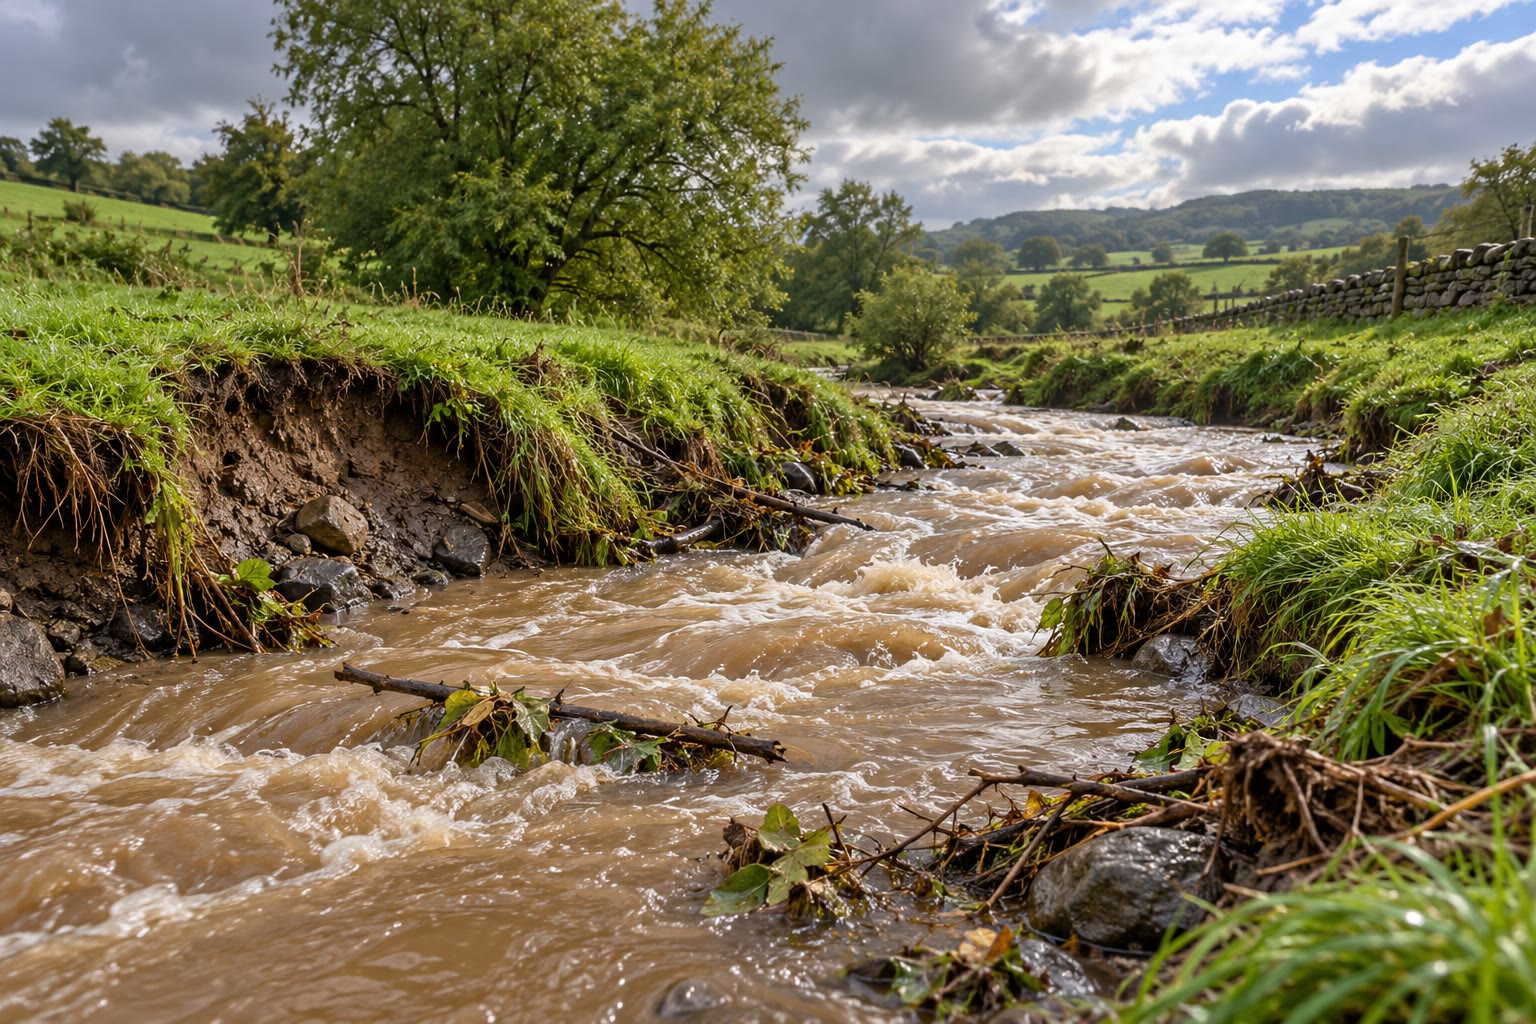
\includegraphics[width=0.5\linewidth]{images/book1/ai/g5-brown-stream.jpg}

{\small Um riacho na manhã seguinte a uma tempestade: a água está marrom
da \omterm{def:g3:stones-pebbles-sand:sand}{lama} e da \omterm{def:g3:stones-pebbles-sand:sand}{areia} que carrega.}
\end{omfigure}

\begin{recall}
A \omterm{def:g3:stones-pebbles-sand:rock}{rocha} é o material duro da Terra; quebrada em pedaços, ela dá pedras,
\omterm{def:g3:stones-pebbles-sand:pebble}{seixos} arredondados pela água, \omterm{def:g3:stones-pebbles-sand:sand}{areia}, cujos grãos vemos um por um, e \omterm{def:g3:stones-pebbles-sand:sand}{lama},
cujos grãos são pequenos demais para ver (\cref{ch:g3:stones-pebbles-sand}).
Um \omterm{def:g1:landscapes-around-us:water}{rio} corre sem parar num canal comprido, de um terreno mais alto até um
\omterm{def:g1:landscapes-around-us:water}{lago} ou até o \omterm{def:g2:water-on-earth:ocean}{mar} (\cref{ch:g1:landscapes-around-us}). A \omterm{def:g4:clouds-rain-snow:precipitation}{chuva} que cai na
terra escorre para os riachos e os \omterm{def:g1:landscapes-around-us:water}{rios}, que levam a água de volta para o
\omterm{def:g2:water-on-earth:ocean}{mar} (\cref{ch:g2:water-on-earth}).
\end{recall}

\section{A rocha se quebra no lugar onde está}

Nem a \omterm{def:g3:stones-pebbles-sand:rock}{rocha} mais dura dura para sempre. Onde ela fica exposta, ao sol, à
\omterm{def:g4:clouds-rain-snow:precipitation}{chuva} e à geada, ela vai rachando e se esfarelando devagar.

\begin{definition}[Intemperismo]\label{def:g5:water-shapes-the-land:weathering}
O \emph{intemperismo}\index{intemperismo} é a fragmentação lenta da \omterm{def:g3:stones-pebbles-sand:rock}{rocha} no
lugar onde ela está, pela geada, pela água, pelas raízes das plantas e pelo
calor e pelo frio. A \omterm{def:g3:stones-pebbles-sand:rock}{rocha} se quebra em pedaços, mas os pedaços ficam no lugar.
\end{definition}

A geada é uma das ferramentas mais fortes do \omterm{def:g5:water-shapes-the-land:weathering}{intemperismo}. A água da
\omterm{def:g4:clouds-rain-snow:precipitation}{chuva} se infiltra numa rachadura fina da \omterm{def:g3:stones-pebbles-sand:rock}{rocha}. Numa noite fria, ela
congela, e, quando a água congela, ela ocupa um pouco mais de espaço: o
gelo empurra os lados da rachadura e a abre só mais um pouquinho. No dia
seguinte o gelo derrete, entra mais água, e na noite seguinte ela congela
de novo. Depois de muitos invernos, um pedaço de \omterm{def:g3:stones-pebbles-sand:rock}{rocha} se solta.

\begin{omfigure}
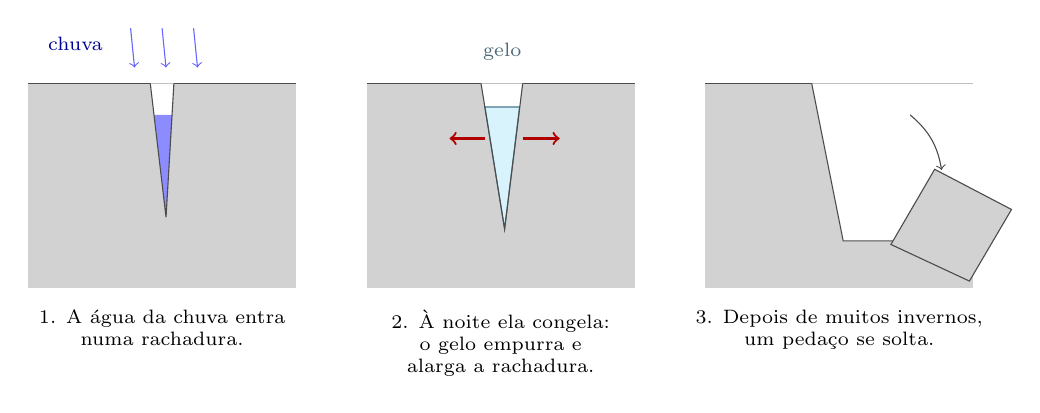
\begin{tikzpicture}[x=1cm, y=1cm, font=\scriptsize]
  \foreach \i/\t in {0/{1. A água da chuva entra\\numa rachadura.},
                     4.3/{2. À noite ela congela:\\o gelo empurra e\\alarga a rachadura.},
                     8.6/{3. Depois de muitos invernos,\\um pedaço se solta.}} {
    \begin{scope}[xshift=\i cm]
      \fill[gray!35] (0,0) rectangle (3.4,2.6);
      \draw[gray!60!black] (0,2.6) -- (3.4,2.6);
      \node[align=center, anchor=north] at (1.7,-0.15) {\t};
    \end{scope}
  }
  % panel 1: thin crack with water
  \fill[white] (1.55,2.6) -- (1.75,0.9) -- (1.85,2.6) -- cycle;
  \fill[blue!45] (1.6,2.2) -- (1.75,0.9) -- (1.83,2.2) -- cycle;
  \draw[gray!60!black] (1.55,2.6) -- (1.75,0.9) -- (1.85,2.6);
  \foreach \x in {1.3,1.7,2.1} \draw[blue!60, ->] (\x,3.3) -- (\x+0.05,2.8);
  \node[blue!60!black] at (0.6,3.1) {chuva};
  % panel 2: wider crack with ice
  \begin{scope}[xshift=4.3cm]
    \fill[white] (1.45,2.6) -- (1.75,0.75) -- (1.98,2.6) -- cycle;
    \fill[cyan!15] (1.5,2.3) -- (1.75,0.75) -- (1.94,2.3) -- cycle;
    \draw[cyan!50!black] (1.5,2.3) -- (1.75,0.75) -- (1.94,2.3) -- cycle;
    \draw[gray!60!black] (1.45,2.6) -- (1.75,0.75) -- (1.98,2.6);
    \draw[red!70!black, thick, <-] (1.05,1.9) -- (1.5,1.9);
    \draw[red!70!black, thick, ->] (1.98,1.9) -- (2.45,1.9);
    \node[cyan!40!black] at (1.72,3.0) {gelo};
  \end{scope}
  % panel 3: broken block
  \begin{scope}[xshift=8.6cm]
    \fill[white] (1.35,2.6) -- (1.75,0.6) -- (3.4,0.6) -- (3.4,2.6) -- cycle;
    \draw[gray!60!black] (1.35,2.6) -- (1.75,0.6) -- (3.4,0.6);
    \fill[gray!35, draw=gray!60!black, rotate around={-25:(2.9,0.3)}]
      (2.3,0.3) -- (2.4,1.4) -- (3.5,1.35) -- (3.4,0.3) -- cycle;
    \draw[gray!60!black, ->] (2.6,2.2) to[bend left=20] (3.0,1.5);
  \end{scope}
\end{tikzpicture}

{\small A geada quebra a \omterm{def:g3:stones-pebbles-sand:rock}{rocha}. A cada noite de geada, o gelo numa
rachadura empurra um pouco; depois de muitos invernos, a rachadura fica
larga o bastante para um pedaço se soltar.}
\end{omfigure}

Embaixo de um paredão de \omterm{def:g3:stones-pebbles-sand:rock}{rocha} nua, no alto das \omterm{def:g1:landscapes-around-us:landform}{montanhas}, os pedaços
soltos pela geada escorregam e rolam encosta abaixo, e se acumulam numa
rampa de pedras pontudas. Elas não são arredondadas: nenhuma água as fez
rolar ainda.

\begin{omfigure}
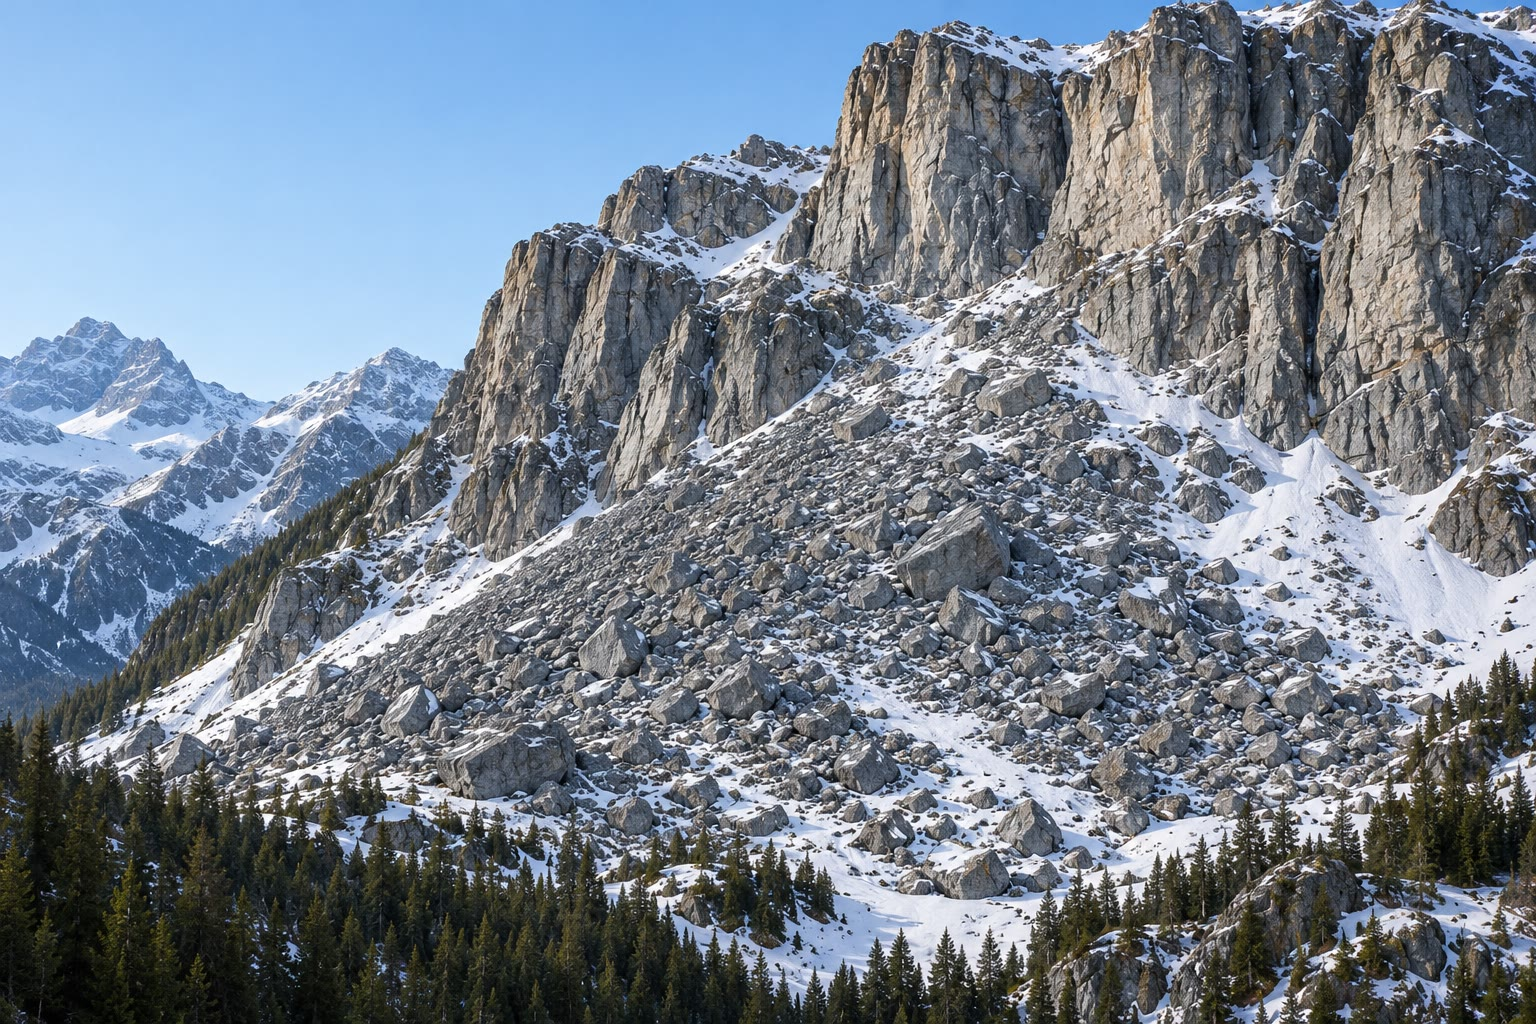
\includegraphics[width=0.5\linewidth]{images/book1/ai/g5-frost-scree.jpg}

{\small Embaixo de um paredão de \omterm{def:g1:landscapes-around-us:landform}{montanha}, uma rampa de pedras pontudas
soltas pela geada, vista do outro lado do \omterm{def:g1:landscapes-around-us:landform}{vale}.}
\end{omfigure}

As plantas também ajudam. Uma raiz de árvore entra numa rachadura e, à
medida que engrossa ano após ano, racha a \omterm{def:g3:stones-pebbles-sand:rock}{rocha} como uma cunha lenta. A
própria água da \omterm{def:g4:clouds-rain-snow:precipitation}{chuva} amolece devagar algumas \omterm{def:g3:stones-pebbles-sand:rock}{rochas} e as transforma em
argila e \omterm{def:g3:stones-pebbles-sand:sand}{areia}: é assim que o solo ganha os seus grãos minerais.

\section{A água leva os pedaços embora}

Depois que a \omterm{def:g3:stones-pebbles-sand:rock}{rocha} se quebra, os pedaços podem se mover. Alguma coisa precisa carregá-los.

\begin{definition}[Erosão]\label{def:g5:water-shapes-the-land:erosion}
A \emph{erosão}\index{erosao@erosão} é o desgaste do terreno e o transporte
dos pedaços de \omterm{def:g3:stones-pebbles-sand:rock}{rocha}, sobretudo pela água corrente, mas também pelo vento,
pelo gelo e pelas ondas do \omterm{def:g2:water-on-earth:ocean}{mar}.
\end{definition}

A água corrente faz a maior parte do trabalho. A \omterm{def:g4:clouds-rain-snow:precipitation}{chuva} lava o solo e os
grãos encosta abaixo até os riachos; os riachos arrancam mais das suas
próprias margens, como fez o riacho de Tom e Lena depois da tempestade.
Quanto mais rápido a água corre, mais ela consegue carregar, e maiores são
os pedaços que ela consegue mover: um riacho calmo só carrega \omterm{def:g3:stones-pebbles-sand:sand}{lama} fina;
um riacho em cheia rola \omterm{def:g3:stones-pebbles-sand:pebble}{seixos} e até matacões pelo seu leito.

No caminho, as pedras batem umas nas outras e no leito. Os cantos se
quebram, e elas viram \omterm{def:g3:stones-pebbles-sand:pebble}{seixos} arredondados, depois grãos cada vez menores:
\omterm{def:g3:stones-pebbles-sand:sand}{areia} e \omterm{def:g3:stones-pebbles-sand:sand}{lama}.

O vento faz o mesmo trabalho nos lugares secos, onde nada segura a \omterm{def:g3:stones-pebbles-sand:sand}{areia}:
ele a sopra e forma dunas. O gelo, nas \omterm{def:g1:landscapes-around-us:landform}{montanhas} e perto dos \omterm{def:g3:continents-and-oceans:poles}{polos}, arrasta
pedras embaixo do seu enorme peso. No \omterm{def:g1:landscapes-around-us:water}{litoral}, as ondas batem nos
penhascos e fazem os \omterm{def:g3:stones-pebbles-sand:pebble}{seixos} da praia rolar para lá e para cá.

\begin{remark}[Quanto?]\label{rem:g5:water-shapes-the-land:how-much}
Juntos, todos os \omterm{def:g1:landscapes-around-us:water}{rios} do mundo levam mais de 12 bilhões de toneladas de
\omterm{def:g3:stones-pebbles-sand:sand}{lama} e de \omterm{def:g3:stones-pebbles-sand:sand}{areia} para o \omterm{def:g2:water-on-earth:ocean}{mar} todo ano. Isso dá cerca de um bilhão de
toneladas por mês.
% ledger: syvitski:modern-flux
\end{remark}

\section{A água deposita os pedaços}

Um \omterm{def:g1:landscapes-around-us:water}{rio} não consegue carregar a sua carga para sempre. Onde ele fica mais
lento, ele não tem mais força para mover os seus grãos maiores, e eles se
depositam no leito.

\begin{definition}[Deposição]\label{def:g5:water-shapes-the-land:deposition}
A \emph{deposição}\index{deposicao@deposição} é o assentamento dos pedaços de \omterm{def:g3:stones-pebbles-sand:rock}{rocha}
carregados pela água, pelo vento ou pelo gelo, onde eles ficam mais lentos e param.
\end{definition}

Os pedaços mais pesados se depositam primeiro: os \omterm{def:g3:stones-pebbles-sand:pebble}{seixos} caem onde a
correnteza diminui um pouco, a \omterm{def:g3:stones-pebbles-sand:sand}{areia} onde ela diminui mais, e a \omterm{def:g3:stones-pebbles-sand:sand}{lama} fina
só onde a água está quase parada, num \omterm{def:g1:landscapes-around-us:water}{lago} ou no \omterm{def:g2:water-on-earth:ocean}{mar}. É por isso que o
leito de um \omterm{def:g1:landscapes-around-us:water}{rio} é de \omterm{def:g3:stones-pebbles-sand:pebble}{seixos} nas \omterm{def:g1:landscapes-around-us:landform}{montanhas} e de \omterm{def:g3:stones-pebbles-sand:sand}{areia} ou de \omterm{def:g3:stones-pebbles-sand:sand}{lama} perto do \omterm{def:g2:water-on-earth:ocean}{mar}.

O \omterm{def:g5:water-shapes-the-land:weathering}{intemperismo}, a \omterm{def:g5:water-shapes-the-land:erosion}{erosão} e a \omterm{def:g5:water-shapes-the-land:deposition}{deposição} são três etapas de uma mesma longa
viagem: a \omterm{def:g3:stones-pebbles-sand:rock}{rocha} se quebra no lugar onde está, os seus pedaços são levados
embora e são depositados em outro lugar. Devagar, a água leva as
\omterm{def:g1:landscapes-around-us:landform}{montanhas}, grão por grão, até as \omterm{def:g1:landscapes-around-us:landform}{planícies} e o \omterm{def:g2:water-on-earth:ocean}{mar}.

\begin{method}[Dar nome ao que a água faz]\label{met:g5:water-shapes-the-land:naming}
Para dar nome ao que está acontecendo com a \omterm{def:g3:stones-pebbles-sand:rock}{rocha} numa imagem ou numa
história, faça três perguntas:
\begin{enumerate}
  \item A \omterm{def:g3:stones-pebbles-sand:rock}{rocha} está sendo quebrada, mas os pedaços ficam onde estão? Isso
        é o \emph{\omterm{def:g5:water-shapes-the-land:weathering}{intemperismo}}.
  \item Os pedaços estão sendo desgastados e levados embora? Isso é a
        \emph{\omterm{def:g5:water-shapes-the-land:erosion}{erosão}}.
  \item Os pedaços estão se depositando e se acumulando? Isso é a
        \emph{\omterm{def:g5:water-shapes-the-land:deposition}{deposição}}.
\end{enumerate}
\end{method}

\begin{example}[O riacho depois da tempestade]\label{ex:g5:water-shapes-the-land:stream}
A água marrom do riacho de Tom e Lena carrega \omterm{def:g3:stones-pebbles-sand:sand}{lama} arrancada das suas
margens: isso é \omterm{def:g5:water-shapes-the-land:erosion}{erosão}. Uma semana depois, o riacho está limpo de novo, e
uma camada fina de \omterm{def:g3:stones-pebbles-sand:sand}{lama} cobre o fundo da poça calma no fim do pátio: isso
é \omterm{def:g5:water-shapes-the-land:deposition}{deposição}.
\end{example}

\section{Um rio da nascente à foz}

Todo \omterm{def:g1:landscapes-around-us:water}{rio} tem um começo e um fim.

\begin{definition}[Nascente, foz e afluente]\label{def:g5:water-shapes-the-land:source-mouth}
A \emph{nascente}\index{nascente (de um rio)} de um \omterm{def:g1:landscapes-around-us:water}{rio} é o lugar onde ele
começa: uma fonte, uma geleira que derrete, ou uma terra alta e encharcada
onde nascem muitos riachinhos. A sua \emph{foz}\index{foz (de um rio)} é o lugar
onde ele termina, desaguando no \omterm{def:g2:water-on-earth:ocean}{mar}, num \omterm{def:g1:landscapes-around-us:water}{lago} ou num \omterm{def:g1:landscapes-around-us:water}{rio} maior. Um
\emph{afluente}\index{afluente} é um \omterm{def:g1:landscapes-around-us:water}{rio} menor que deságua num \omterm{def:g1:landscapes-around-us:water}{rio} maior.
\end{definition}

Ao longo do caminho, um \omterm{def:g1:landscapes-around-us:water}{rio} muda. Dividimos o seu comprimento em três
partes: o curso superior, o curso médio e o curso inferior.

\begin{omfigure}
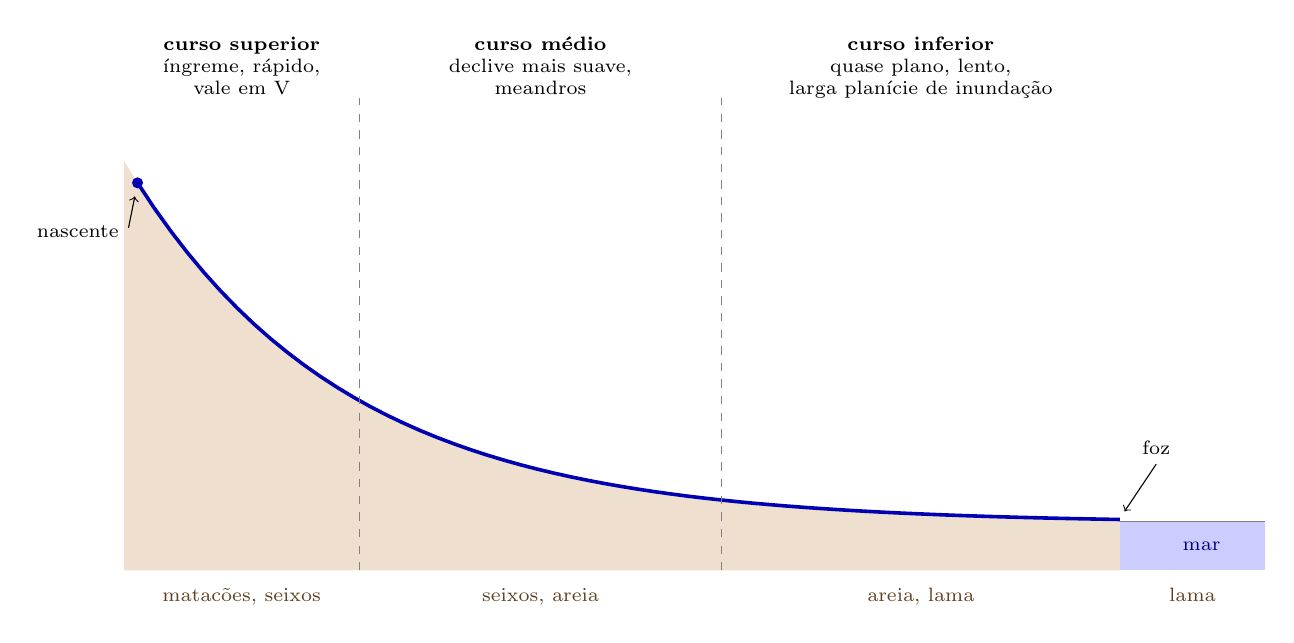
\begin{tikzpicture}[x=1.15cm, y=1cm, font=\scriptsize]
  % ground
  \fill[brown!25] (0,-0.6) -- plot[domain=0:11, samples=60]
    (\x,{4.6*exp(-\x/2.4)}) -- (11,-0.6) -- cycle;
  % sea
  \fill[blue!20] (11,-0.6) rectangle (12.6,0.02);
  \draw[blue!70!black, line width=1.3pt] plot[domain=0.15:11, samples=60]
    (\x,{4.6*exp(-\x/2.4)});
  \draw[gray] (11,0.02) -- (12.6,0.02);
  \node[blue!50!black] at (11.9,-0.3) {mar};
  % course limits
  \foreach \x in {2.6,6.6} \draw[gray, dashed] (\x,-0.6) -- (\x,5.4);
  \node[align=center, anchor=north] at (1.3,6.3) {\textbf{curso superior}\\íngreme, rápido,\\vale em V};
  \node[align=center, anchor=north] at (4.6,6.3) {\textbf{curso médio}\\declive mais suave,\\meandros};
  \node[align=center, anchor=north] at (8.8,6.3) {\textbf{curso inferior}\\quase plano, lento,\\larga planície de inundação};
  % source and mouth
  \fill[blue!70!black] (0.15,{4.6*exp(-0.15/2.4)}) circle (2pt);
  \node[anchor=east] at (0.05,3.7) {nascente};
  \draw[->] (0.05,3.75) -- (0.12,4.15);
  \node[anchor=south] at (11.4,0.75) {foz};
  \draw[->] (11.4,0.75) -- (11.05,0.15);
  % grain sizes
  \node[anchor=north, align=center, text=brown!50!black] at (1.3,-0.7) {matacões, seixos};
  \node[anchor=north, align=center, text=brown!50!black] at (4.6,-0.7) {seixos, areia};
  \node[anchor=north, align=center, text=brown!50!black] at (8.8,-0.7) {areia, lama};
  \node[anchor=north, align=center, text=brown!50!black] at (11.8,-0.7) {lama};
\end{tikzpicture}

{\small O perfil longitudinal de um \omterm{def:g1:landscapes-around-us:water}{rio}, da \omterm{def:g5:water-shapes-the-land:source-mouth}{nascente} à \omterm{def:g5:water-shapes-the-land:source-mouth}{foz} (as alturas estão
muito exageradas). Embaixo: o que há no seu leito.}
\end{omfigure}

No seu \emph{curso superior}, nas \omterm{def:g1:landscapes-around-us:landform}{montanhas}, o \omterm{def:g1:landscapes-around-us:water}{rio} é jovem e íngreme. A
água desce com pressa, rola matacões pelo leito e escava a \omterm{def:g3:stones-pebbles-sand:rock}{rocha} para
baixo. Ele cava um \omterm{def:g1:landscapes-around-us:landform}{vale} estreito, de encostas íngremes, com a forma da
letra V.

No seu \emph{curso médio}, o declive é mais suave. O \omterm{def:g1:landscapes-around-us:water}{rio} vai de um lado
para o outro, fazendo grandes curvas.

\begin{definition}[Meandro]\label{def:g5:water-shapes-the-land:meander}
Um \emph{meandro}\index{meandro} é uma curva de um \omterm{def:g1:landscapes-around-us:water}{rio} que serpenteia pelo
fundo plano de um \omterm{def:g1:landscapes-around-us:landform}{vale}.
\end{definition}

Um \omterm{def:g5:water-shapes-the-land:meander}{meandro} não fica parado: ele se desloca. Do lado de fora de cada curva,
a água corre rápida e funda: ela escava a margem, que vira um pequeno
barranco. Do lado de dentro da curva, a água corre devagar: ela deixa \omterm{def:g3:stones-pebbles-sand:sand}{areia}
e \omterm{def:g3:stones-pebbles-sand:pebble}{cascalho}, que formam uma praia suave. Ano após ano, a margem de fora
recua e a praia de dentro cresce, e a curva fica cada vez mais aberta.

\begin{omfigure}
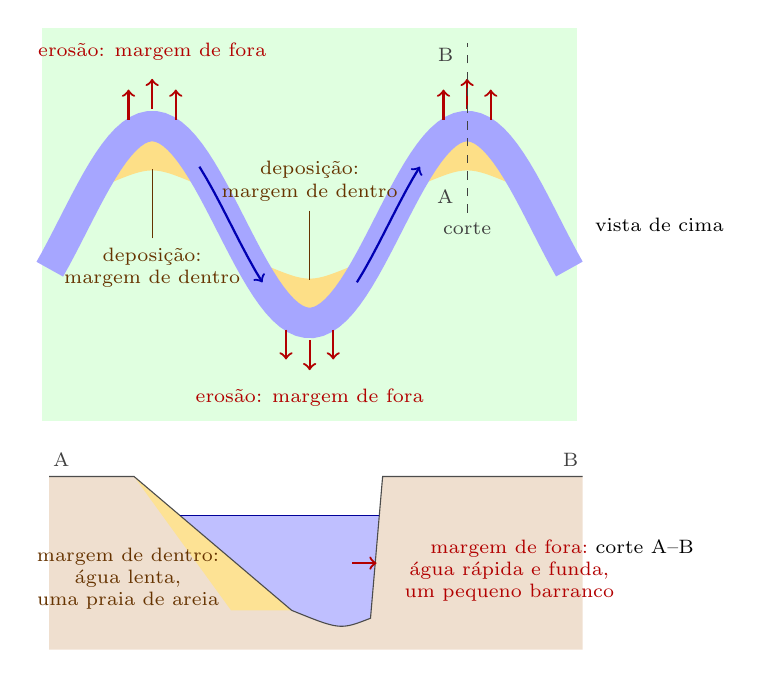
\begin{tikzpicture}[x=1cm, y=1cm, font=\scriptsize]
  % ---- map view ----
  \fill[green!12] (-0.4,-2.5) rectangle (6.4,2.5);
  % sand on the inner banks (drawn first, the river covers its edge)
  \foreach \c/\s in {1/1, 3/-1, 5/1}
    \fill[yellow!50!orange!45] (\c-0.6,\s*0.5) .. controls (\c,\s*1.5) ..
      (\c+0.6,\s*0.5) .. controls (\c,\s*0.75) .. cycle;
  % the river
  \draw[blue!35, line width=11pt] plot[domain=-0.3:6.3, samples=90]
    (\x,{1.25*sin(\x*90)});
  \draw[blue!70!black, ->, thick] plot[domain=1.6:2.4, samples=10]
    (\x,{1.25*sin(\x*90)});
  \draw[blue!70!black, ->, thick] plot[domain=3.6:4.4, samples=10]
    (\x,{1.25*sin(\x*90)});
  % erosion on the outer banks
  \foreach \c/\s in {1/1, 3/-1, 5/1}
    \foreach \d in {-0.3,0,0.3}
      \draw[red!70!black, thick, ->] (\c+\d,{\s*(1.25*cos(\d*90)+0.22)})
        -- (\c+\d,{\s*(1.25*cos(\d*90)+0.6)});
  \node[red!70!black] at (1,2.2) {erosão: margem de fora};
  \node[red!70!black] at (3,-2.2) {erosão: margem de fora};
  \node[orange!40!black, align=center] (d1) at (1,-0.55) {deposição:\\margem de dentro};
  \node[orange!40!black, align=center] (d2) at (3,0.55) {deposição:\\margem de dentro};
  \draw[orange!40!black] (d1.north) -- (1,0.7);
  \draw[orange!40!black] (d2.south) -- (3,-0.7);
  \draw[gray!50!black, dashed] (5,0.15) -- (5,2.3);
  \node[gray!50!black, anchor=north] at (5,0.15) {corte};
  \node[gray!50!black, anchor=east] at (4.95,0.35) {A};
  \node[gray!50!black, anchor=east] at (4.95,2.15) {B};
  \node[anchor=west] at (6.5,0) {vista de cima};
  % ---- cut ----
  \begin{scope}[yshift=-4.1cm, xscale=0.77]
    \fill[brown!25] (-0.4,-1.3) -- (-0.4,0.9) -- (1,0.9) -- (3.6,-0.8)
      .. controls (4.4,-1.05) .. (4.9,-0.9) -- (5.1,0.9) -- (8.4,0.9)
      -- (8.4,-1.3) -- cycle;
    \fill[blue!25] (1.75,0.4) -- (3.6,-0.8) .. controls (4.4,-1.05) .. (4.9,-0.9)
      -- (5.04,0.4) -- cycle;
    \fill[yellow!50!orange!40] (1,0.9) -- (3.6,-0.8) -- (2.6,-0.8) -- cycle;
    \draw[gray!60!black] (-0.4,0.9) -- (1,0.9) -- (3.6,-0.8)
      .. controls (4.4,-1.05) .. (4.9,-0.9) -- (5.1,0.9) -- (8.4,0.9);
    \draw[blue!60!black] (1.75,0.4) -- (5.04,0.4);
    \node[orange!40!black, align=center] at (0.9,-0.4) {margem de dentro:\\água lenta,\\uma praia de areia};
    \node[red!70!black, align=center, anchor=west] at (5.3,-0.3) {margem de fora:\\água rápida e funda,\\um pequeno barranco};
    \draw[red!70!black, thick, ->] (4.6,-0.2) -- (5.0,-0.2);
    \node[gray!50!black, anchor=south] at (-0.2,0.9) {A};
    \node[gray!50!black, anchor=south] at (8.2,0.9) {B};
    \node[anchor=west] at (8.45,0) {corte A--B};
  \end{scope}
\end{tikzpicture}

{\small Um \omterm{def:g5:water-shapes-the-land:meander}{meandro} visto de cima e cortado ao longo da linha tracejada A--B.
A água desgasta a margem de fora de cada curva e deixa \omterm{def:g3:stones-pebbles-sand:sand}{areia} na margem de
dentro: a curva se desloca devagar.}
\end{omfigure}

Às vezes duas curvas crescem tanto que ficam muito próximas e, durante uma
cheia, o \omterm{def:g1:landscapes-around-us:water}{rio} rompe a estreita faixa de terra entre elas e pega o atalho. A
curva antiga fica para trás como um \omterm{def:g1:landscapes-around-us:water}{lago} curvo.

\begin{omfigure}
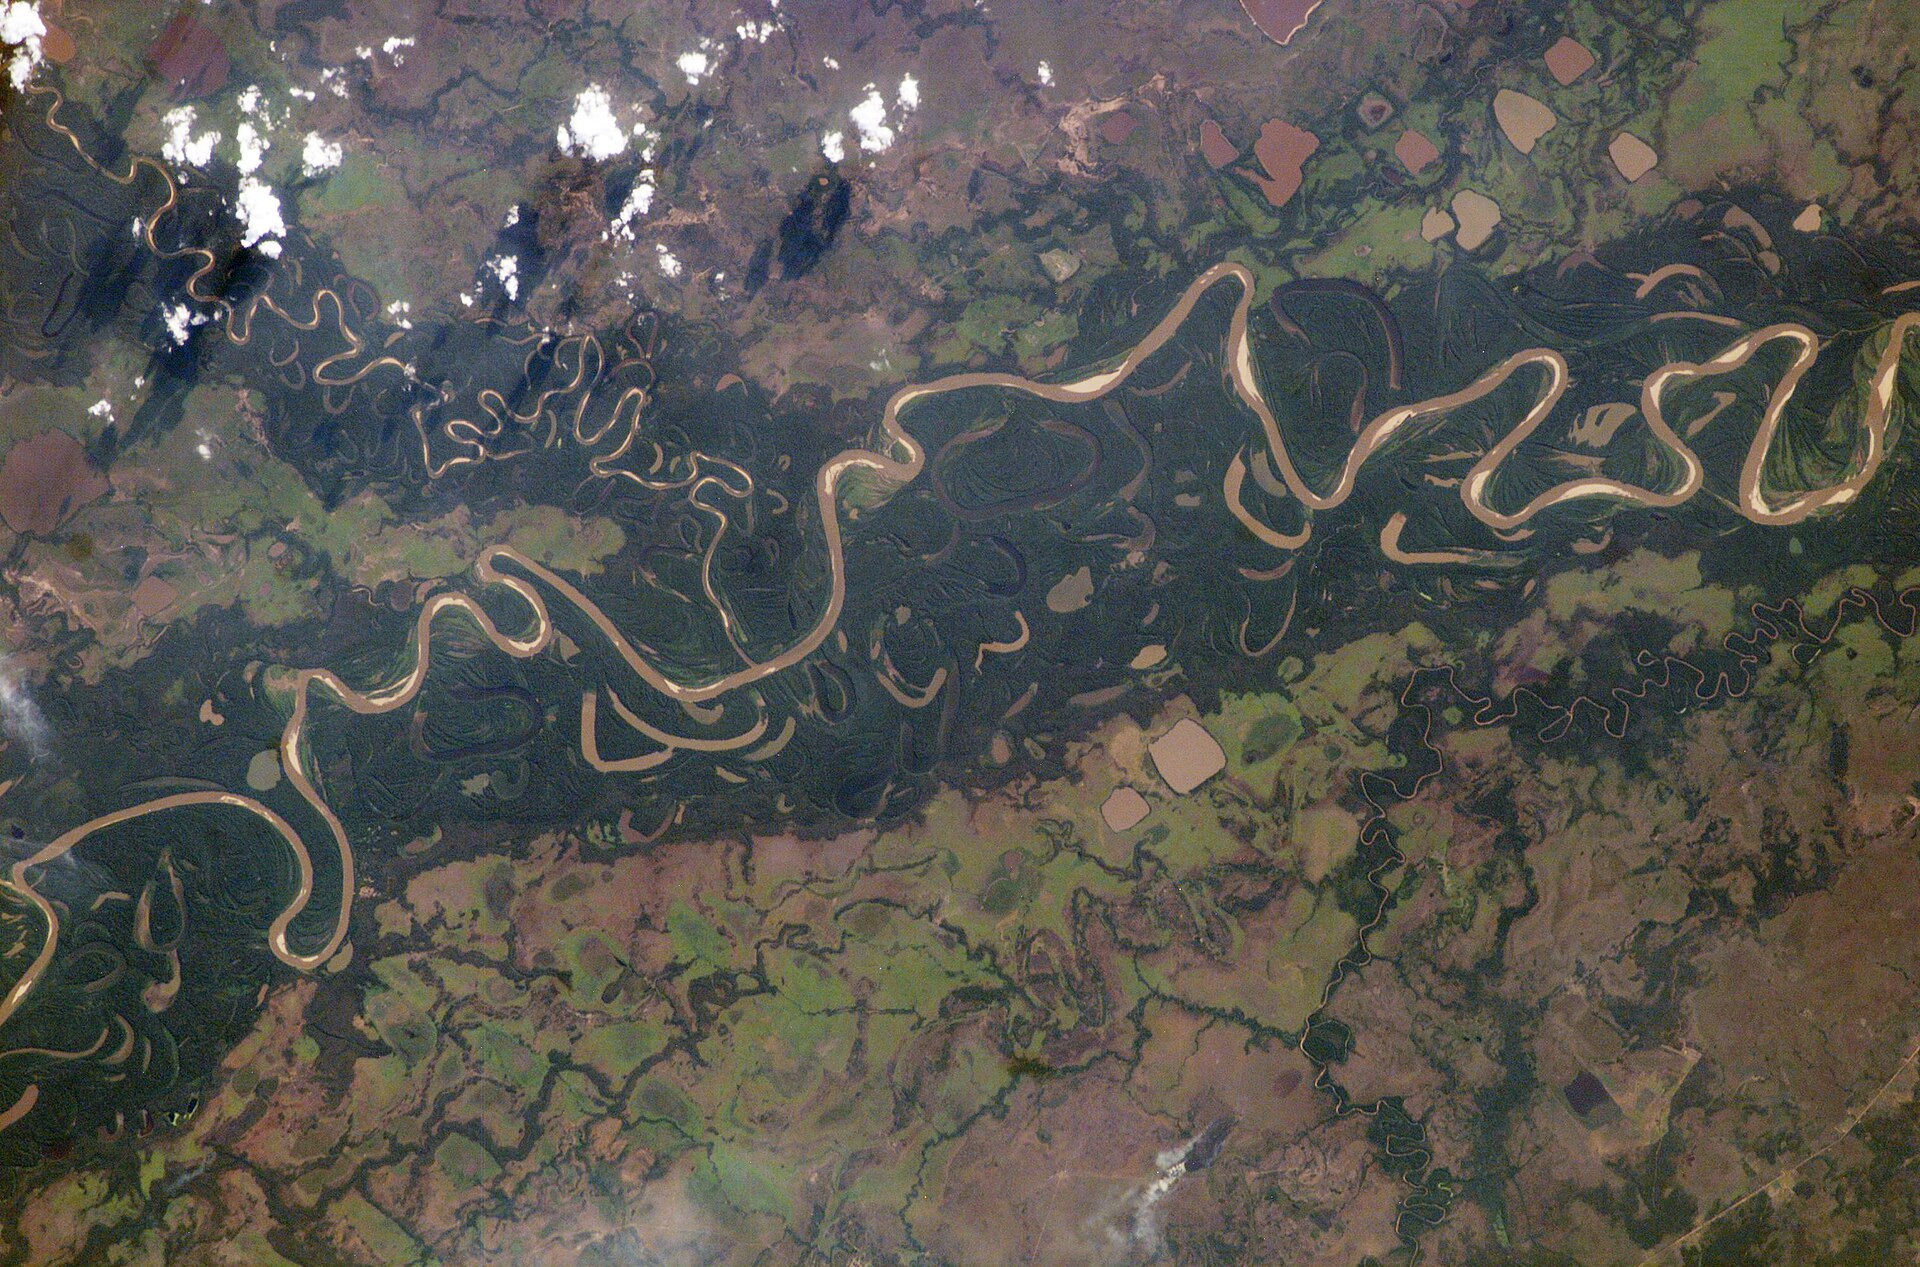
\includegraphics[width=0.52\linewidth]{images/book1/g5-mamore-meanders.jpg}

{\small O \omterm{def:g1:landscapes-around-us:water}{rio} Mamoré, nas terras baixas da Bolívia, na América do Sul, visto
da Estação Espacial Internacional. O \omterm{def:g1:landscapes-around-us:water}{rio} marrom serpenteia em \omterm{def:g5:water-shapes-the-land:meander}{meandros} pela
floresta. Foto: NASA (domínio público).}\label{fig:g5:water-shapes-the-land:mamore}
% ledger: nasa:mamore-meanders
\end{omfigure}

No seu \emph{curso inferior}, o terreno é quase plano. O \omterm{def:g1:landscapes-around-us:water}{rio} corre devagar
por um fundo de \omterm{def:g1:landscapes-around-us:landform}{vale} largo e plano, feito da \omterm{def:g3:stones-pebbles-sand:sand}{lama} e da \omterm{def:g3:stones-pebbles-sand:sand}{areia} que ele mesmo
depositou ao longo de muito tempo.

\begin{omfigure}
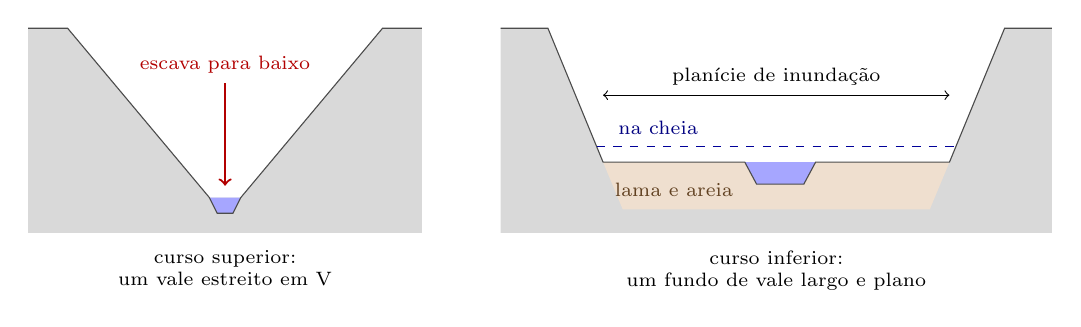
\begin{tikzpicture}[x=1cm, y=1cm, font=\scriptsize]
  % V-shaped valley
  \fill[gray!30] (0,0) -- (0,2.6) -- (0.5,2.6) -- (2.3,0.45) -- (2.7,0.45)
    -- (4.5,2.6) -- (5,2.6) -- (5,0) -- cycle;
  \fill[blue!35] (2.3,0.45) -- (2.4,0.25) -- (2.6,0.25) -- (2.7,0.45) -- cycle;
  \draw[gray!60!black] (0,2.6) -- (0.5,2.6) -- (2.3,0.45) -- (2.4,0.25)
    -- (2.6,0.25) -- (2.7,0.45) -- (4.5,2.6) -- (5,2.6);
  \draw[red!70!black, thick, ->] (2.5,1.9) -- (2.5,0.6);
  \node[red!70!black, anchor=south] at (2.5,1.9) {escava para baixo};
  \node[align=center, anchor=north] at (2.5,-0.1) {curso superior:\\um vale estreito em V};
  % floodplain
  \begin{scope}[xshift=6cm]
    \fill[gray!30] (0,0) -- (0,2.6) -- (0.6,2.6) -- (1.3,0.9) -- (5.7,0.9)
      -- (6.4,2.6) -- (7,2.6) -- (7,0) -- cycle;
    \fill[brown!25] (1.3,0.9) -- (1.55,0.3) -- (5.45,0.3) -- (5.7,0.9) -- cycle;
    \fill[blue!35] (3.1,0.9) -- (3.25,0.62) -- (3.85,0.62) -- (4,0.9) -- cycle;
    \draw[gray!60!black] (0,2.6) -- (0.6,2.6) -- (1.3,0.9) -- (3.1,0.9)
      -- (3.25,0.62) -- (3.85,0.62) -- (4,0.9) -- (5.7,0.9) -- (6.4,2.6) -- (7,2.6);
    \draw[blue!60!black, dashed] (1.22,1.1) -- (5.78,1.1);
    \node[blue!50!black, anchor=south] at (2.0,1.12) {na cheia};
    \node[brown!50!black] at (2.2,0.55) {lama e areia};
    \draw[<->] (1.3,1.75) -- (5.7,1.75);
    \node[anchor=south] at (3.5,1.75) {planície de inundação};
    \node[align=center, anchor=north] at (3.5,-0.1) {curso inferior:\\um fundo de vale largo e plano};
  \end{scope}
\end{tikzpicture}

{\small O \omterm{def:g1:landscapes-around-us:landform}{vale} cortado transversalmente, nas \omterm{def:g1:landscapes-around-us:landform}{montanhas} e perto do \omterm{def:g2:water-on-earth:ocean}{mar} (não na
mesma escala). Na cheia, o \omterm{def:g1:landscapes-around-us:water}{rio} se espalha por toda a sua \omterm{def:g5:water-shapes-the-land:flood}{planície de inundação}.}
\end{omfigure}

Por fim, o \omterm{def:g1:landscapes-around-us:water}{rio} chega à sua \omterm{def:g5:water-shapes-the-land:source-mouth}{foz}. Ali a água fica quase parada, e o \omterm{def:g1:landscapes-around-us:water}{rio} deixa
o resto da sua carga. Onde as ondas e as marés do \omterm{def:g2:water-on-earth:ocean}{mar} são fracas demais
para levar tudo embora, a \omterm{def:g3:stones-pebbles-sand:sand}{lama} e a \omterm{def:g3:stones-pebbles-sand:sand}{areia} se acumulam, e uma terra nova
avança sobre o \omterm{def:g2:water-on-earth:ocean}{mar}.

\begin{definition}[Delta]\label{def:g5:water-shapes-the-land:delta}
Um \emph{delta}\index{delta} é uma terra nova e plana construída por um \omterm{def:g1:landscapes-around-us:water}{rio}
na sua \omterm{def:g5:water-shapes-the-land:source-mouth}{foz}, com a \omterm{def:g3:stones-pebbles-sand:sand}{lama} e a \omterm{def:g3:stones-pebbles-sand:sand}{areia} que ele deposita. O \omterm{def:g1:landscapes-around-us:water}{rio} se divide em
vários braços que se espalham sobre ela, muitas vezes em forma de leque.
\end{definition}

O nome vem da letra grega $\Delta$ (\omterm{def:g5:water-shapes-the-land:delta}{delta}), um triângulo, porque o \omterm{def:g5:water-shapes-the-land:delta}{delta}
do Nilo, no Egito, tem essa forma.

Alguns \omterm{def:g1:landscapes-around-us:water}{rios} terminam sem \omterm{def:g5:water-shapes-the-land:delta}{delta}. Onde ondas e marés fortes levam a \omterm{def:g3:stones-pebbles-sand:sand}{lama}
embora, o \omterm{def:g1:landscapes-around-us:water}{rio} termina numa \omterm{def:g5:water-shapes-the-land:source-mouth}{foz} larga, em forma de funil, por onde o \omterm{def:g2:water-on-earth:ocean}{mar}
entra e sai com as marés: um \emph{estuário}.

\begin{omfigure}
\begin{minipage}[b]{0.55\linewidth}\centering
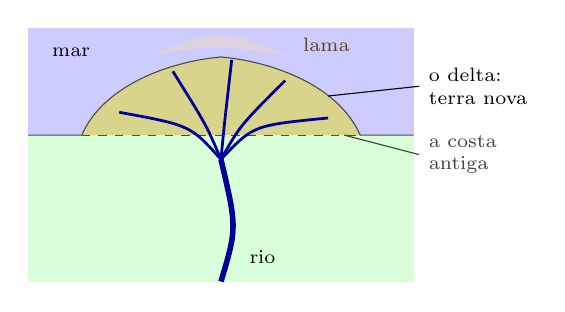
\begin{tikzpicture}[x=0.68cm, y=0.62cm, font=\scriptsize]
  \fill[blue!20] (-3.6,1.4) rectangle (3.6,3.6);
  \fill[green!15] (-3.6,-1.6) rectangle (3.6,1.4);
  % delta
  \fill[olive!35] (-2.6,1.4) .. controls (-2.2,2.4) and (-1,2.9)
    .. (0,3.0) .. controls (1,2.9) and (2.2,2.4) .. (2.6,1.4) -- cycle;
  \draw[gray!60!black] (-3.6,1.4) -- (-2.6,1.4) .. controls (-2.2,2.4) and
    (-1,2.9) .. (0,3.0) .. controls (1,2.9) and (2.2,2.4) .. (2.6,1.4) -- (3.6,1.4);
  \draw[gray!60!black, dashed] (-2.6,1.4) -- (2.6,1.4);
  % river and branches
  \draw[blue!60!black, line width=2pt] (0,-1.6) .. controls (0.3,-0.5) .. (0,0.9);
  \foreach \e in {-1.9,-0.9,0.2,1.2,2.0}
    \draw[blue!60!black, line width=1pt] (0,0.9) .. controls (\e*0.3,1.6) ..
      (\e,{2.95-0.3*\e*\e});
  % mud plume
  \fill[brown!30, opacity=0.5] (-1.3,3.05) .. controls (0,3.6) .. (1.3,3.0)
    .. controls (0,3.25) .. cycle;
  \node[align=center] at (-2.8,3.1) {mar};
  \node[anchor=west, brown!50!black] at (1.35,3.25) {lama};
  \node[anchor=west, align=left] at (3.7,2.4) {o delta:\\terra nova};
  \draw (3.7,2.4) -- (2.0,2.2);
  \node[anchor=west, align=left, gray!50!black] at (3.7,1.0) {a costa\\antiga};
  \draw[gray!50!black] (3.7,1.0) -- (2.3,1.4);
  \node[anchor=west] at (0.35,-1.1) {rio};
\end{tikzpicture}
\end{minipage}\hfill
\begin{minipage}[b]{0.3\linewidth}\centering
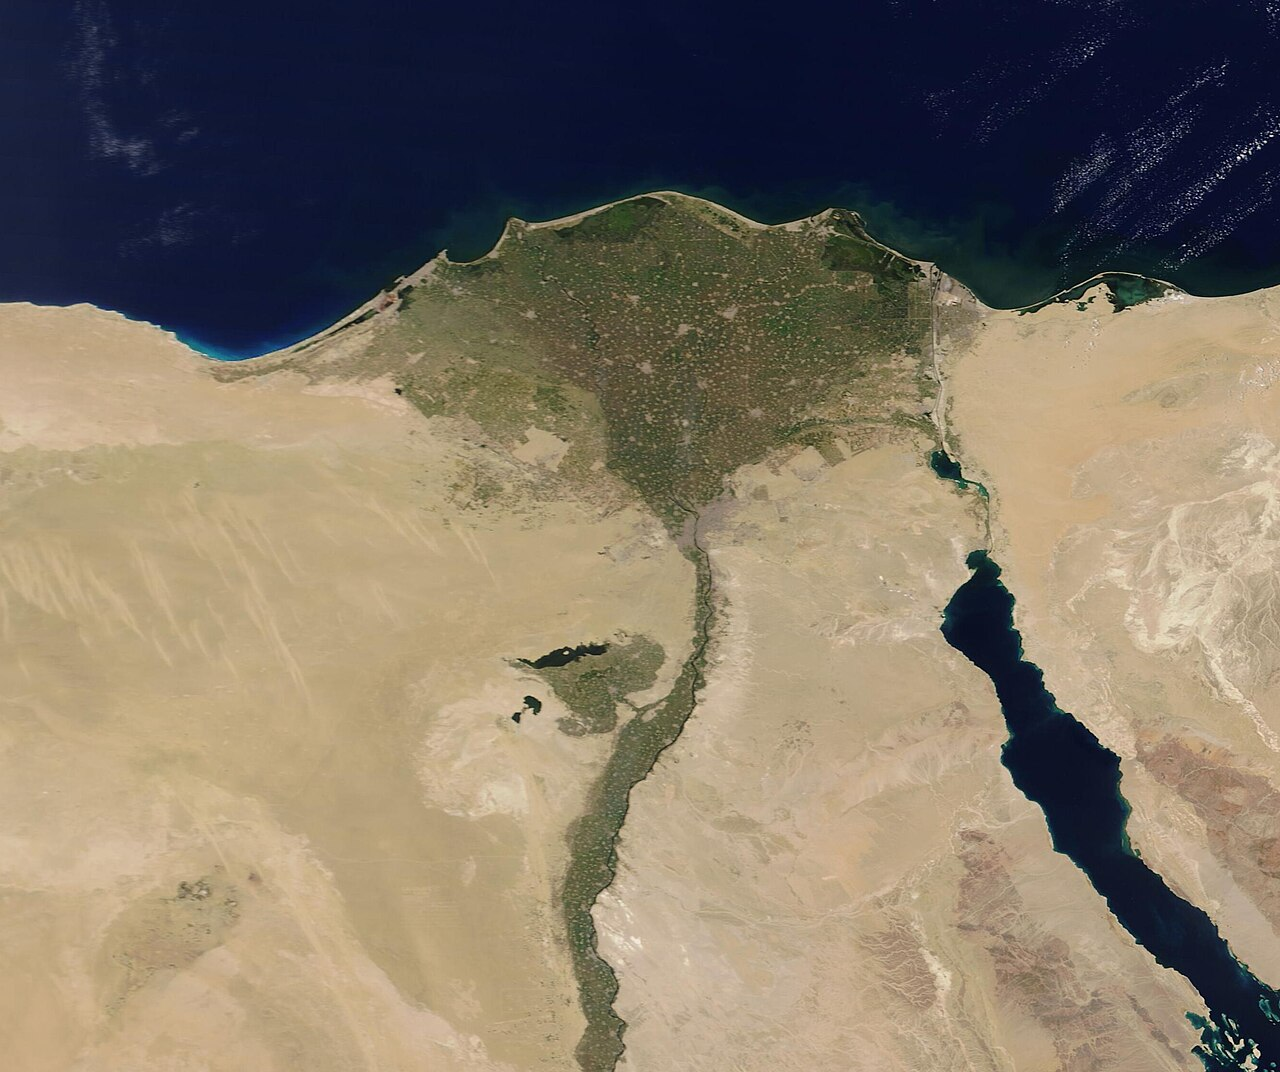
\includegraphics[width=\linewidth]{images/book1/g5-nile-delta-modis.jpg}
\end{minipage}

{\small À esquerda: um \omterm{def:g5:water-shapes-the-land:delta}{delta} visto de cima; a \omterm{def:g3:stones-pebbles-sand:sand}{lama} e a \omterm{def:g3:stones-pebbles-sand:sand}{areia} depositadas
pelos braços constroem uma terra nova além da costa antiga. À direita: o
\omterm{def:g5:water-shapes-the-land:delta}{delta} do Nilo, no Egito, visto de um satélite (o \omterm{def:g2:water-on-earth:ocean}{mar} fica no alto): um
leque verde de plantações sobre a \omterm{def:g3:stones-pebbles-sand:sand}{lama} do \omterm{def:g1:landscapes-around-us:water}{rio}, no meio do deserto. Foto:
NASA (domínio público).}
% ledger: nasa:nile-delta-modis
\end{omfigure}

\section{As inundações}

Depois de muitos dias de \omterm{def:g4:clouds-rain-snow:precipitation}{chuva}, ou quando a \omterm{def:g4:clouds-rain-snow:precipitation}{neve} derrete depressa na
primavera, um \omterm{def:g1:landscapes-around-us:water}{rio} recebe mais água do que o seu canal consegue conter.

\begin{definition}[Inundação e planície de inundação]\label{def:g5:water-shapes-the-land:flood}
Uma \emph{inundação}\index{inundacao@inundação} acontece quando a água cobre uma
terra que normalmente fica seca. Um \omterm{def:g1:landscapes-around-us:water}{rio} transborda quando sobe acima das
suas margens e se espalha pela terra plana dos dois lados. Essa terra
plana, que o \omterm{def:g1:landscapes-around-us:water}{rio} cobre de vez em quando, é a sua \emph{planície de
inundação}\index{planicie de inundacao@planície de inundação}.
\end{definition}

\begin{omfigure}
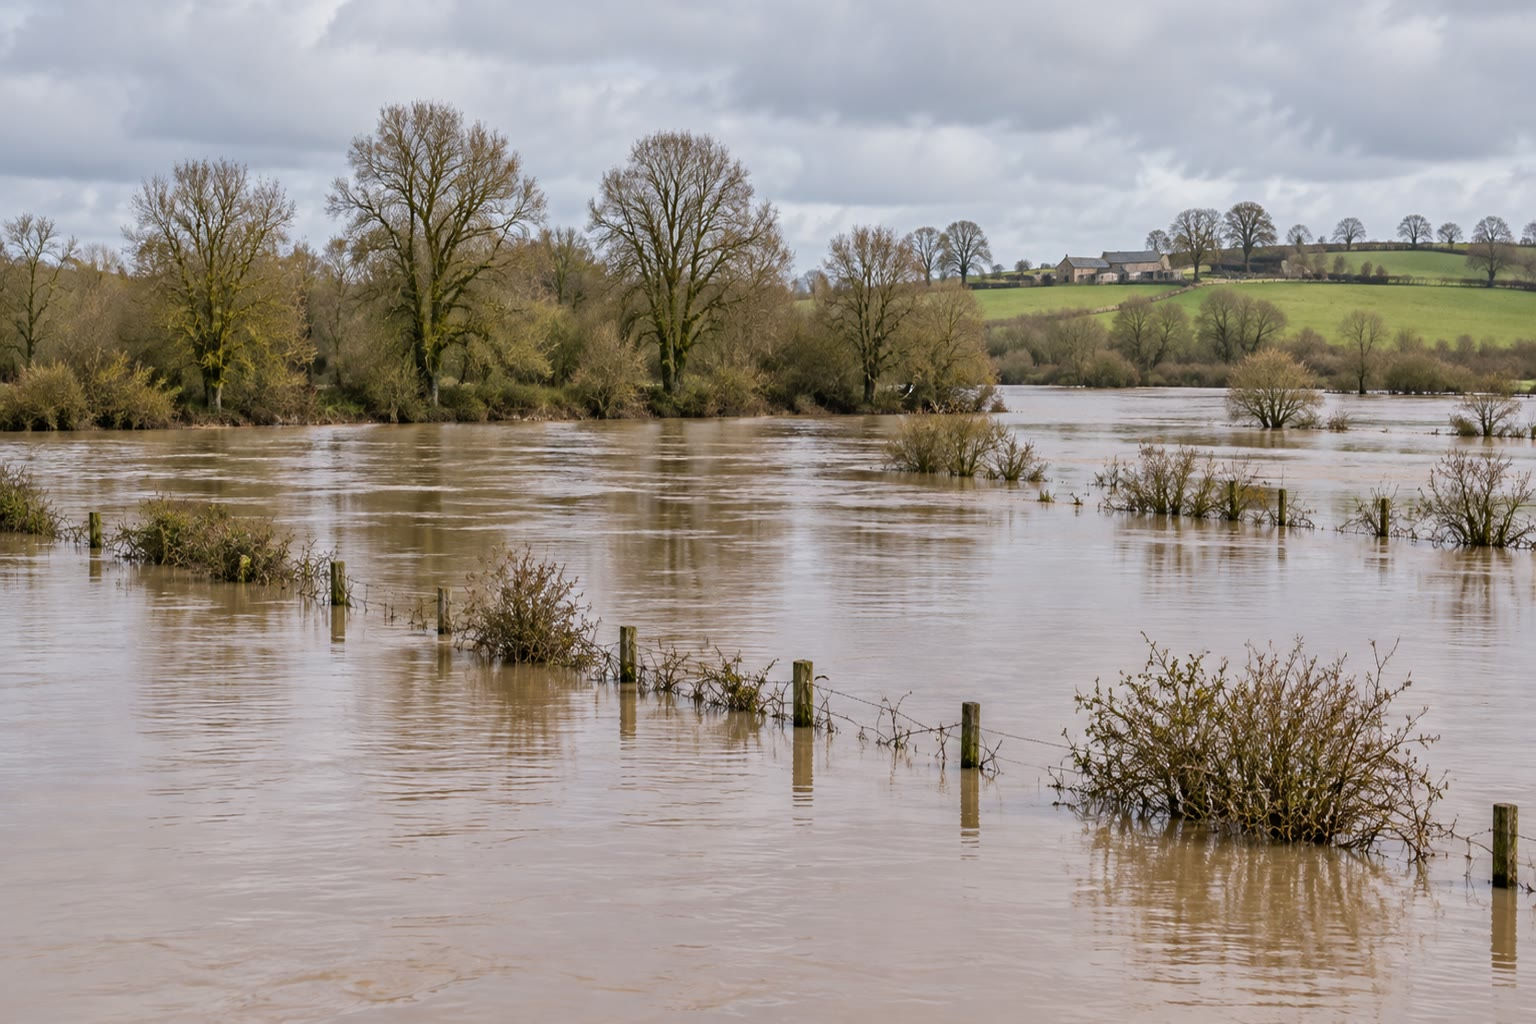
\includegraphics[width=0.5\linewidth]{images/book1/ai/g5-flooded-meadow.jpg}

{\small Um pasto embaixo da água de uma \omterm{def:g5:water-shapes-the-land:flood}{inundação}, depois de dias de \omterm{def:g4:clouds-rain-snow:precipitation}{chuva}.
A fileira de árvores marca a margem habitual do \omterm{def:g1:landscapes-around-us:water}{rio}; o sítio fica num
terreno mais alto.}
\end{omfigure}

Um \omterm{def:g1:landscapes-around-us:water}{rio} que transborda não está fazendo nada de estranho: ele está fazendo
o que os \omterm{def:g1:landscapes-around-us:water}{rios} sempre fizeram. A \omterm{def:g5:water-shapes-the-land:flood}{planície de inundação} é o território dele.
Na verdade, foi o \omterm{def:g1:landscapes-around-us:water}{rio} que a construiu: cada cheia deixa uma camada fina de
\omterm{def:g3:stones-pebbles-sand:sand}{lama} sobre os campos, e é por isso que as \omterm{def:g5:water-shapes-the-land:flood}{planícies de inundação} têm um
solo tão rico. Antigamente, os agricultores do Egito esperavam a cheia
anual do Nilo, que regava os seus campos e lhes trazia \omterm{def:g3:stones-pebbles-sand:sand}{lama} nova.

Mas uma \omterm{def:g5:water-shapes-the-land:flood}{inundação} é perigosa para quem mora na \omterm{def:g5:water-shapes-the-land:flood}{planície de inundação}. As
casas construídas ali podem ficar cheias de água, e a água rápida de uma
enchente pode arrastar carros e pessoas. Uma cidade sensata constrói em
terreno mais alto e deixa a \omterm{def:g5:water-shapes-the-land:flood}{planície de inundação} para plantações, pastos
e parques. No \cref{ch:g5:natural-hazards} vamos ver como as pessoas se
preparam para as \omterm{def:g5:water-shapes-the-land:flood}{inundações} e se protegem.

\begin{safety}
Nunca ande, pedale ou brinque na água de uma enchente, e nunca chegue perto
de um \omterm{def:g1:landscapes-around-us:water}{rio} em cheia: a água é mais forte e mais funda do que parece, e pode
esconder buracos e bueiros abertos. Fique longe até os adultos responsáveis
dizerem que não há mais perigo.
\end{safety}

\section{Exercícios}

\begin{exercise}[$\star$]\label{exo:g5:water-shapes-the-land:1}
Dê o nome do processo: \omterm{def:g5:water-shapes-the-land:weathering}{intemperismo}, \omterm{def:g5:water-shapes-the-land:erosion}{erosão} ou \omterm{def:g5:water-shapes-the-land:deposition}{deposição}?
\begin{enumerate}
  \item[(a)] O gelo numa rachadura racha uma \omterm{def:g3:stones-pebbles-sand:rock}{rocha} numa \omterm{def:g1:landscapes-around-us:landform}{montanha}.
  \item[(b)] Um \omterm{def:g1:landscapes-around-us:water}{rio} em cheia leva embora a \omterm{def:g3:stones-pebbles-sand:sand}{areia} das suas margens.
  \item[(c)] Uma camada de \omterm{def:g3:stones-pebbles-sand:sand}{lama} se deposita no fundo de um \omterm{def:g1:landscapes-around-us:water}{lago} calmo.
  \item[(d)] Uma raiz de árvore racha um muro de pedra.
\end{enumerate}
\end{exercise}

\begin{exercise}[$\star$]\label{exo:g5:water-shapes-the-land:2}
O que é a \omterm{def:g5:water-shapes-the-land:source-mouth}{nascente} de um \omterm{def:g1:landscapes-around-us:water}{rio}? O que é a sua \omterm{def:g5:water-shapes-the-land:source-mouth}{foz}? O que é um \omterm{def:g5:water-shapes-the-land:source-mouth}{afluente}?
\end{exercise}

\begin{exercise}[$\star$]\label{exo:g5:water-shapes-the-land:3}
Coloque estas partes de um \omterm{def:g1:landscapes-around-us:water}{rio} em ordem, da \omterm{def:g5:water-shapes-the-land:source-mouth}{nascente} até o \omterm{def:g2:water-on-earth:ocean}{mar}: os
\omterm{def:g5:water-shapes-the-land:meander}{meandros}; o \omterm{def:g5:water-shapes-the-land:delta}{delta}; o \omterm{def:g1:landscapes-around-us:landform}{vale} estreito em V; a \omterm{def:g5:water-shapes-the-land:source-mouth}{nascente}.
\end{exercise}

\begin{exercise}[$\star$]\label{exo:g5:water-shapes-the-land:4}
Verdadeiro ou falso? Explique.
\begin{enumerate}
  \item[(a)] A \omterm{def:g3:stones-pebbles-sand:rock}{rocha} dura nunca muda.
  \item[(b)] Um \omterm{def:g1:landscapes-around-us:water}{rio} rápido consegue carregar pedras maiores que um \omterm{def:g1:landscapes-around-us:water}{rio} lento.
  \item[(c)] A \omterm{def:g3:stones-pebbles-sand:sand}{lama} mais fina se deposita primeiro, perto da \omterm{def:g5:water-shapes-the-land:source-mouth}{nascente}.
\end{enumerate}
\end{exercise}

\begin{exercise}[$\star$]\label{exo:g5:water-shapes-the-land:5}
Veja uma curva de um \omterm{def:g1:landscapes-around-us:water}{rio} vista de cima.

\begin{center}
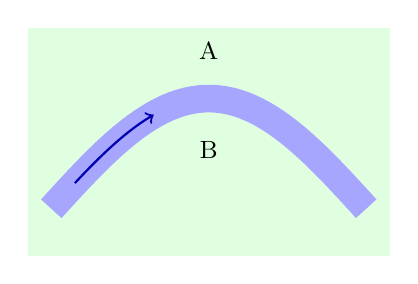
\begin{tikzpicture}[x=1cm, y=1cm, font=\small]
  \fill[green!12] (-0.3,-0.6) rectangle (4.3,2.3);
  \draw[blue!35, line width=10pt] plot[domain=0:4, samples=50]
    (\x,{1.4*sin(\x*45)});
  \draw[blue!70!black, ->, thick] plot[domain=0.3:1.3, samples=20]
    (\x,{1.4*sin(\x*45)});
  \node at (2,2.0) {A};
  \node at (2,0.75) {B};
\end{tikzpicture}
\end{center}
Em que margem, A ou B, o \omterm{def:g1:landscapes-around-us:water}{rio} desgasta o terreno? Em que margem ele deixa
\omterm{def:g3:stones-pebbles-sand:sand}{areia}?
\end{exercise}

\begin{exercise}[$\star$]\label{exo:g5:water-shapes-the-land:6}
Nas \omterm{def:g1:landscapes-around-us:landform}{montanhas}, o leito de um \omterm{def:g1:landscapes-around-us:water}{rio} é coberto de pedras grandes. Perto do
\omterm{def:g2:water-on-earth:ocean}{mar}, ele é coberto de \omterm{def:g3:stones-pebbles-sand:sand}{areia} e de \omterm{def:g3:stones-pebbles-sand:sand}{lama}. Por quê?
\end{exercise}

\begin{exercise}[$\star\star$]\label{exo:g5:water-shapes-the-land:7}
Um \omterm{def:g1:landscapes-around-us:water}{rio} tem 600 quilômetros de comprimento. O seu curso superior é o
primeiro $\frac{1}{6}$ do seu comprimento, e o seu curso médio, a metade
seguinte, $\frac{1}{2}$.
\begin{enumerate}
  \item[(a)] Qual é o comprimento do curso superior? E do curso médio?
  \item[(b)] Qual é o comprimento do curso inferior? Que fração do \omterm{def:g1:landscapes-around-us:water}{rio} ele
        representa?
\end{enumerate}
\end{exercise}

\begin{exercise}[$\star\star$]\label{exo:g5:water-shapes-the-land:8}
Observe de novo a foto do \omterm{def:g1:landscapes-around-us:water}{rio} Mamoré vista da estação espacial, na
página~\pageref{fig:g5:water-shapes-the-land:mamore}. O que são as manchas claras do lado de dentro
das curvas? O que são os \omterm{def:g1:landscapes-around-us:water}{lagos} curvos e escuros ao lado do \omterm{def:g1:landscapes-around-us:water}{rio}? Como eles se formaram?
\end{exercise}

\begin{exercise}[$\star\star$]\label{exo:g5:water-shapes-the-land:9}
Uma cidade quer construir uma escola nova nos pastos verdes e planos ao
lado do seu \omterm{def:g1:landscapes-around-us:water}{rio}, porque ali o terreno é plano e barato. O que você diria à
câmara municipal? Use as palavras \emph{\omterm{def:g5:water-shapes-the-land:flood}{inundação}} e \emph{\omterm{def:g5:water-shapes-the-land:flood}{planície de inundação}}.
\end{exercise}

\begin{exercise}[$\star\star$]\label{exo:g5:water-shapes-the-land:10}
Os \omterm{def:g1:landscapes-around-us:water}{rios} do mundo levam cerca de 12 bilhões de toneladas de \omterm{def:g3:stones-pebbles-sand:sand}{lama} e de \omterm{def:g3:stones-pebbles-sand:sand}{areia}
para o \omterm{def:g2:water-on-earth:ocean}{mar} todo ano.
\begin{enumerate}
  \item[(a)] Quantas toneladas isso dá por mês, em média?
  \item[(b)] Um caminhão grande carrega 10 toneladas. Quantas cargas de
        caminhão seriam necessárias para levar a \omterm{def:g3:stones-pebbles-sand:sand}{lama} e a \omterm{def:g3:stones-pebbles-sand:sand}{areia} de um mês?
\end{enumerate}
\end{exercise}

\begin{exercise}[$\star\star\star$]\label{exo:g5:water-shapes-the-land:11}
Conte a história de um grão de \omterm{def:g3:stones-pebbles-sand:sand}{areia}. Ele começa como parte de uma \omterm{def:g3:stones-pebbles-sand:rock}{rocha}
no alto de uma \omterm{def:g1:landscapes-around-us:landform}{montanha} e termina, muitos anos depois, num \omterm{def:g5:water-shapes-the-land:delta}{delta}. Use as
palavras \emph{\omterm{def:g5:water-shapes-the-land:weathering}{intemperismo}}, \emph{\omterm{def:g5:water-shapes-the-land:erosion}{erosão}} e \emph{\omterm{def:g5:water-shapes-the-land:deposition}{deposição}}, e diga o
que acontece com o grão no curso superior, no curso médio e no curso
inferior do \omterm{def:g1:landscapes-around-us:water}{rio}.
\end{exercise}
